\section{Related Works}

First of all, we need to go over some definitions for this part of our paper. In this section, we will be speaking of metrics, which are measures of some property of a piece of software. There are several metrics that can be calculated in software, but we will mainly be talking about \emph{ownership} and \emph{focus} in the following sections.\\
Ownership is defined as \emph{a general term used to describe whether one person has responsibility for a software component, or if there is no one clearly responsible developer}\cite{DontTouchMyCode}. In our study, we also define a component as a set of software artifacts (mainly files), and a contribution as a modification on a given component.

\subsection{How Developers Drive Software Evolution\\ \textit{T. Girba, A. Kuhn, M. Seeberger, S. Ducasse (IWPSE'2005)}}

The evolution of a project may sometimes be surprising, and developer knowledge becomes more and more important as the projects becomes more and more complex. Therefore it may sometimes be useful to know which developer might have the best knowledge of each file in the project in order to assign tasks such as bugfixes, or even to ask for help on the matter.
This paper defines the \emph{ownership} metric, as the degree to which a developer is the "owner" of a file at a given time during the project's development\cite{Girba2005}.

In order to achieve this, they use the CVS logs of a project in order to calculate a number of metrics, and determine which developer might be considered as most knowledgeable of a file in the project, and designate him as owner of that file.
They also created the following visualisation of ownership during a project's lifetime:

\begin{figure}[H]
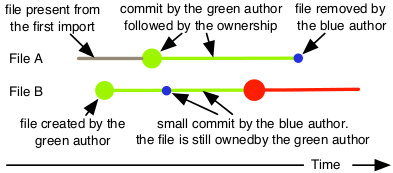
\includegraphics[keepaspectratio=true,scale=0.5]{./resources/girba2005.png}~
\caption{commit map}
\label{fig:commit_map}
\end{figure}

When this visualisation is applied to an entire project, it becomes possible to detect behavioural pattern between developers. See appendix[1].

Given that CVS is a file-based versionning system, a developer will be considered an owner of a file if he has written/edited the highest amount of lines within that file. This leaves the system open to inappropriate changes of ownership if for instance a developer decides to reformat the code, leading to a file owner who actually has little knowledge of the file.

On the other hand, this visualisation did allow them to detect behavioural patterns amoung the developers of projects:
\begin{itemize}
\item \textbf{Monologue:} One developer is the owner of a portion of the project for a time.
\item \textbf{Dialogue:} Two or more developerss take ownership alternatively of a portion of the project.
\item \textbf{Teamwork:} A kind of Dialogue, with a quick succession of commits by several developers.
\item \textbf{Silence:} Little to no activity during a period.
\item \textbf{Takeover:} A developer suddenly takes ownership on a large portion of the project.
\item \textbf{Familiarisation:} Like a Takeover, but over a longer period of time.
\item \textbf{Expansion:} A Takeover followed by the addition of files to the project.
\item \textbf{Cleanup:} The opposite of Expansion, a developer deletes files or lines of code.
\item \textbf{Bugfix:} A small punctual change.
\item \textbf{Edit:} Non functionnal changes (formatting, comments, ect...)
\end{itemize}

With these events, we can determine how the project was developed, who was the main developer, and more.
\subsection{How Developers Develop Features\\ \textit{T. Girba, O. Greevy, S. Ducasse (CSMR'2007)}}

In 2007 the same team published this paper\cite{Girba2007}, on a similar subject as the previous. This time, they shifted their focus towards ownership of features as well as files. Indeed, the standard point of view, i.e ownership of packages, is how developers think about their code. However domain analysts and users are more likely to think in terms of features. Studying this metric could be useful to link the external and functionnal aspect of a project with its internal structure.
The visualisation displays the ownership of files within the project's features, which are also structurally linked. The following image is a representation of this visualisation on a program that is designed to manage a mobile phone:

\begin{figure}[H]
\centering
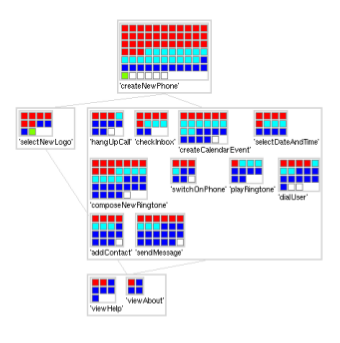
\includegraphics[width=0.4\textwidth]{./resources/girba2007.png}~
\caption{Ownership map By Feature}
\label{fig:ownership_map_by_feature}
\end{figure}

This visualisation makes it possible to determine whom one might ask in order to help resolve a bug in a feature, rather than having to identify which file belongs to which feature, as one would need to do with the previous paper's visualisation.~\ref{fig:annex_ownership_outsight}.
The goal was also to determine if developers tend to develop features or functionnal blocks. They determined that project contributions were mainly distributed on a package boundary.

\subsection{Dual Ecological Measures of Focus in Software Development\\ \textit{D. Posnett, R. D’Souza, R. Devanbu, V. Filkov (ICSE'2013)}}

This paper took an interesting approach to measuring the relation between component and developer. Using a biological analogy with prey/predator type relationships between components and developers\cite{Posnett}. That is to say that modules prey on a developer's time. Therefore, in this visualisation, we have two points of view. On the one hand, the developers, and the contributions they have made to each component (a larger edge represents more contributions), and on the other hand, we have the components, and the contributions they have received. As in the following figure:

\begin{figure}[H]
\centering
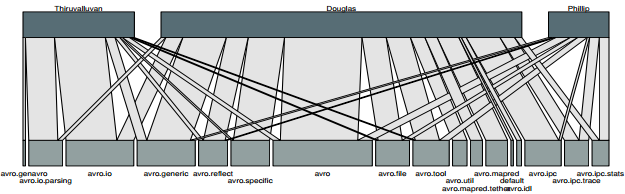
\includegraphics[width=0.5\textwidth]{./resources/focus.png}~
\caption{Ownership map By Feature}
\label{fig:ownership_map_by_feature}
\end{figure}

This paper evokes the notion of Focus, both from the developers' point of view and the components'.
\\[0.4cm]
\textbf{DAF: Developer’s Attention Focus}
\begin{itemize}
\item Human attention and cognition are finite resources. If they are spread across many tasks, we can usually see a degradation in performance, and errors, and thus the quality of work will suffer. This is the same with all things, and especially in software development.
\item This metric is designed to measure how focused a developer is on his work, and thus give an indication of the quality of his work compared to his potential.
\end{itemize}

\textbf{MAF: Module Activity Focus}
\begin{itemize}
\item Measures the degree to which activities on the component are focused.
\end{itemize}

Components are viewed as predators, which hunt developers' cognitive resources. When there is a large amount of contributors on a component, it can "feed" and thus thrive.
Developers are viewed as prey, whose limited cognitive ressources are divided amoung the components that are "hunting" them.

Therefore, a developer with a high amount of commits on a single component will have higher focus, whereas a developer with a large amount of commits on several components will have lower focus.
This gives us an idea of the limitations of ownership, because in the second case, the developer might still be considered as owner of several modules, without having concentrated his efforts on these modules.

However, a developer may have high concentration on a few files in a component, but only made small contributions when compared to other developers working on the same module.
Also, a developer that contributes a few times on a large/popular component will not be as specialised as a developer which has made as many contributions to a smaller component.

Given this information, there a some questions to be raised:
\begin{itemize}
\item What kind of behavioural pattern do the top developers follow?
\item Is there any correlation between a high focus and a low amount of bugs?
\end{itemize}

\textbf{Conclusions:}
\begin{itemize}
\item Project leaders tend to have lower levels of Focus than other Developers.
\item High focus implies less bugs introduced.
\item Increasing the Module Activity Focus (MAF) has a negative impact on the quality of that module.
\end{itemize}

This paper and it's visualisation is what inspired us the most when deciding what kind of visualisation we should create.
